In this section are analyzed some known heuristics algorithms for the TSP problem. An heuristic algorithm doesn’t return the optimal solution of the problem but computes a near optimal solution valuing optimality, accuracy, time speed and completeness. Those kinds of algorithms are mainly used when the computational time of the exact algorithms is too high (mainly because of the size of the input instance) and there is no need for an exact solution.

Heuristic Algorithms are divided into three main categories:
\begin{description}
    \item[Constructive Heuristics:] algorithms that iterates to extend a current partial solution until a complete solution is found, trying to make an improvement at each iteration.
    \item[Refinement Heuristics:] starting from a complete solution (not optimal), it rearranges some edges trying to further improve the current solution.
    \item[Metaheuristics:] high level heuristic algorithms mainly used to escape local optimality and to explore a more vast range of possible solutions.
\end{description}

\section{Constructive Heuristics}
\subsection{Greedy: Nearest Neighbor}
Nearest Neighbour it’s a popular greedy algorithm, easy to implement, and that solves the TSP problem in a sub-optimal way. The algorithm \ref{algo:greedy} usually starts with a single starting node and at each iteration it connects the current node to the closest node not already in the path, repeating this operation until all nodes are connected. It’s easy to notice how in general this kind of algorithm won’t find the shortest route and thus his sub-optimality.

\begin{algorithm}
    \caption{Nearest Neighbour}\label{algo:greedy}
    \begin{algorithmic}[1]
    \Require $G = (V,E), c:E \to \mathbb{R}^+, startNode \in V$
    \Ensure $\text{sub optimal TSP solution}$
    \State $visited \gets \left \{ startNode \right \}$
    \State $current \gets startNode$




    \State $solution \gets$ empty
    \State $cost \gets 0$




    \While{$\left | visited \right | \neq \left | V  \right |$}
    \State $candidate \gets *$ find closest node to current $*$
    \State $cost \gets cost + \operatorname{dist}(current, candidate)$
    \State add $candidate$ to $visited$
    \State add ($current$,$candidate$) edge to $solution$
    \State $current \gets candidate$
    \EndWhile




    \State add ($current$,$startNode$) edge to $solution$
    \State $cost \gets cost + \operatorname{dist}(current, startNode)$


    \end{algorithmic}
\end{algorithm}

This algorithm has complexity $O(n^2)$ since it needs to scan at most $n$ nodes for each node in the graph. At fig. \ref{fig:greedy} one can better understand how the algorithm works.

\begin{figure}[!h]
    \centering
    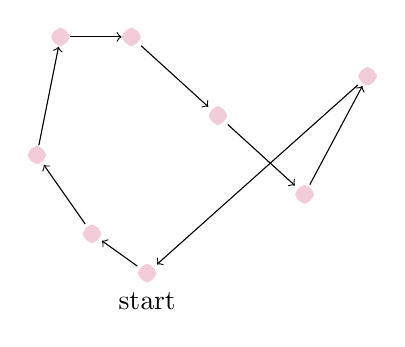
\begin{tikzpicture}
        \tikzstyle{city} = [fill=purple!20,rounded corners]


        \node[city] (A) at (1.3,4.0){};
        \node[city] (B) at (1.6,5.5){};
        \node[city,label=below:start] (C) at (2.7,2.5){};
        \node[city] (D) at (4.7,3.5){};
        \node[city] (E) at (2.0,3.0){};
        \node[city] (F) at (2.5,5.5){};
        \node[city] (G) at (3.6,4.5){};
        \node[city] (H) at (5.5,5){};


        %\draw[->] (C.west) -- (E.east);
        %\draw[->] (B.south) -- (A.east);
        \draw[->] (C) edge (E) (E) edge (A) (A) edge (B) (B) edge (F) (F) edge (G) (G) edge (D) (D) edge (H) (H) edge (C);

    \end{tikzpicture}
    \caption{Example of Nearest Neighbor} \label{fig:greedy}
\end{figure}

To slightly improve this greedy algorithm performance, in our implementation we actually preferred a multistart approach. The algorithm is called multiple times within a time limit and at each iteration a random $startNode$ is used as the starting node. In this way, at each iteration we obtain different solutions with different costs and when the time is up, at the end of the run, only the best solution (the one with minimal cost) is returned in output.

\subsubsection*{The Grasp Variant}
The Greedy Randomized Adaptive Search Procedure (GRASP) is a technique that introduces randomization in the choices of the greedy algorithms.
Applied to the Nearest Neighbor algorithm, it actually works by adding a certain probability value during the running of it and this slightly modifies its behavior of improvement of the current solution.

At each iteration, instead of choosing the nearest node to the current one, we have a certain probability of choosing the second nearest node. That way we can add some randomness to the algorithm and this can actually improve the overall optimality of the final solution.
Obviously even this variant has been implemented and runs similarly to the multistart Nearest Neighbor algorithm within a time limit, and with different starting nodes at each iteration.

\subsection{Extra-Mileage: Farthest Insertion}
The Farthest Insertion heuristic described in algorithm \ref{algo:extramileage}, also called Extra-Mileage heuristic, unlike the Nearest Neighbor algorithm, doesn’t need a starting node, instead starts by connecting the farthest nodes in the graph as an initial cycle. Because of that it is defined as a deterministic method, meaning that it will always return the same solution over the same input instance.

\begin{figure}[!h]
    \centering
    \begin{tikzpicture}
        \tikzstyle{city} = [fill=purple!20,rounded corners]


        \node[city] (A) at (1,5){};
        \node[city] (B) at (2,4){};
        \node[city,label=above:h] (C) at (3,7){};
        \node[city,label=below:j] (D) at (4,1){};
        \node[city,label=above:i] (E) at (6,8){};
        \node[city] (F) at (7,3){};
        \node[city] (G) at (9,6){};


    


        \draw[->] (D) edge[bend right] node [right] {} (E);
        \draw[->] (E) edge[bend right] node [right] {} (D);


        \draw[dashed,->] (E) edge (C) (C) edge (D.west);


    


    \end{tikzpicture}
    \caption{Example of Farthest Insertion} \label{fig:extra}
\end{figure}

\begin{algorithm}[h!]
    \caption{Farthest Insertion}\label{algo:extramileage}
    \begin{algorithmic}[1]
    \Require $G = (V,E), c:E \to \mathbb{R}^+$
    \Ensure $\text{sub optimal TSP solution}$


    \State $solution \gets$ empty
    \State $cost \gets 0$
    \State $visited \gets  *$ find diameter nodes i-j of G $*$
    \State add ($i$,$j$) and ($j$,$i$) edges to $solution$
    \State $cost \gets cost + 2 c_{ij}$
   




    \While{$\left | visited \right | \neq \left | V  \right |$}
    \State $candidate \gets $ generic node h $ \notin visited$
    \State $candidate \gets *$ find edge i-j visited that minimizes $\Delta = c_{ih} + c_{hj} - c_{ij}*$
    \State $cost \gets cost + \Delta$
    \State remove ($i$,$j$) edge to $solution$
    \State add ($i$,$h$) and ($h$,$j$) edges to $solution$
    \State add $candidate$ to $visited$


    \EndWhile






    \end{algorithmic}
\end{algorithm}

The first cycle is initialized using the diameter nodes of the graph, then the algorithm continues by looking for a non selected node as in figure \ref{fig:extra} that if inserted in the solution would result in a lower cost tour than the current one.
That simple metric is computed by testing each non visited node with each possible already existing edge, and then keeping the one with lowest $\Delta = c_{ih} + c_{hj} - c_{ij}$.

The Farthest Insertion algorithm has a worst-case time complexity of $O(n^2)$, where $n$ is the number of nodes. However, it has been shown to perform well in practice and can often produce high-quality solutions that are close to optimal for small and medium-sized instances of the TSP.

\section{Refinement Heuristics}
\subsection{2-OPT Refining}
One of the most popular heuristic algorithms for solving the TSP is the 2-opt algorithm.
The 2-opt algorithm is a local search algorithm that iteratively improves an initial tour by swapping pairs of edges to reduce the length of the tour. The algorithm starts by generating an initial tour, such as one produced by the Nearest Neighbor or Farthest Insertion algorithm. It then repeatedly examines all possible pairs of edges in the tour, and if swapping a pair of edges will reduce the length of the tour, the edges are swapped.

More specifically, the 2-opt algorithm works as follows: first, it generates an initial solution, in our implementation we choose to generate it using the multistart Nearest Neighbor algorithm paired with a GRASP approach. It then examines all pairs of edges $(a,a’)$ and $(b,b’)$, where $a,a’,b$ and $b’$ are distinct nodes. If swapping the edges $(a,a’)$ and $(b,b’)$ will result in a shorter tour, the edges are swapped, and the algorithm continues to search for other pairs of edges to swap. This process is repeated until no further improvements can be made to the tour or until the time limit permits.

To know that a certain swap results in a better solution, the algorithm computes $\Delta \operatorname{c}(a,b) = (c_{ab} + c_{a’b’}) - (c_{aa’} + c_{bb’})$ and if it is negative then we found some good candidates, meaning that the new candidates edges would be shorter than the current ones.

After the swap, the algorithm then changes the order of the successor in the tour to make $b$ connect to $a$ and obtain a new solution, as in fig \ref{fig:2OPT}.

\begin{figure}[!h]
    \centering
    \begin{tikzpicture}
        \tikzstyle{city} = [fill=purple!20,rounded corners]
    
    
        \node[city,label=above:a] (A) at (1,5){};
        \node[city,label=below:b] (B) at (1,1){};
        \node[city,label=above:b'] (C) at (5,5){};
        \node[city,label=below:a'] (D) at (5,1){};
    
    
        \node[city,label=above:a] (E) at (7,5){};
        \node[city,label=below:b] (F) at (7,1){};
        \node[city,label=above:b'] (G) at (11,5){};
        \node[city,label=below:a'] (H) at (11,1){};
    
    
       
    
    
        \draw[dashed,->] (C) edge[bend right] node [right] {} (A);
        \draw[dashed,->] (D) edge[bend left] node [left] {} (B);
    
    
        \draw[dashed,->] (G) edge[bend right] node [right] {} (E);
        \draw[dashed,->,red] (F) edge[bend right] node [left] {} (H);
    
    
        \draw[->] (A) -- (D);
        \draw[->] (B) -- (C);
    
    
        \draw[->] (E) -- (F);
        \draw[->] (H) -- (G);
       
    
    \end{tikzpicture}
    \caption{Example of 2-OPT} \label{fig:2OPT}
\end{figure}

The 2-opt algorithm is known to be effective in practice, and it has been used to solve many large-scale instances of the TSP. The algorithm is relatively efficient, with a time complexity of $O(n^2)$, where $n$ is the number of nodes in the graph.

The same idea goes behind the more general k-OPT Refining algorithm, where instead of swapping only 2 edges at the time, k edges are selected and swapped. For example, 3-opt involves swapping three edges in the tour, while 4-opt involves swapping four edges. By considering larger sets of edges, k-opt can potentially find more optimal solutions than 2-opt, but it is also computationally more expensive.






	



